\section{Experiment 9C: uncertainty-aware compatibility discovery}
\label{sec:experiment9c}

\paragraph{Question and staged gate.}
Experiment 9C asks whether explicit local-identification uncertainty repairs the
short-data and high-noise failures of Experiment 9B. The experiment uses the 9B
seeds 126--135 as a locked development replication. Seeds 136--145 are reserved
as an untouched confirmation set and are opened only if both development
regimes pass. The frozen gate requires the proposed method to remain within 5\%
of Oracle family, strictly improve ordinary point clustering, remain amplitude-
feasible and frozen-stable, and use fewer shared base models than Local. Hard
ARI is retained as a diagnostic rather than a gate because the method explicitly
permits uncertain, soft membership. Privacy remains excluded.

\paragraph{Method.}
For client $i$, the output-error Jacobian $J_i$ is evaluated at the fitted
log-ratios. Given the known output-noise scaling, the Gauss--Newton covariance is
\begin{equation}
 P_i = (J_i^\top J_i)^{-1},
\end{equation}
with eigenvalue regularization only for numerical inversion. The covariance is
mapped into the same normalized log-parameter coordinates used in 9A--9B. A
heteroscedastic mixture then models
\begin{equation}
 z_i \sim \sum_{k=1}^{K}\pi_k\,
 \mathcal{N}(\mu_k,P_i+S_k),
\end{equation}
where $P_i$ is client-specific measurement uncertainty and $S_k$ captures
within-group variation. Generalized EM estimates the weights, means, and full
intrinsic covariances. BIC selects $K\in\{1,\ldots,8\}$ subject to at least ten
hard-assigned training clients per component. For an unseen client, posterior
component probabilities blend the $K$ shared scheduled controllers. Thus the
server retains $K$ base models plus three client membership weights, rather than
a separately learned model for every vehicle.

\begin{table}[htbp]
\centering
\caption{Experiment 9C development results on the two failed 9B regimes.}
\label{tab:experiment9c-results}
\begin{tabular}{lrrrr}
\toprule
Regime and method & Tracking & Mean $K$ & Oracle cost & Point gain\\
\midrule
Short data: Oracle family & 0.007597 & 3.0 & --- & ---\\
Short data: Point-$K$ & 0.011887 & 3.6 & 56.47\% & ---\\
Short data: uncertainty-soft & 0.011810 & 1.0 & 55.45\% & 0.65\%\\
High noise: Oracle family & 0.007632 & 3.0 & --- & ---\\
High noise: Point-$K$ & 0.009715 & 2.3 & 27.29\% & ---\\
High noise: uncertainty-soft & 0.008038 & 2.0 & 5.31\% & 17.27\%\\
\bottomrule
\end{tabular}
\end{table}

\begin{figure}[htbp]
\centering
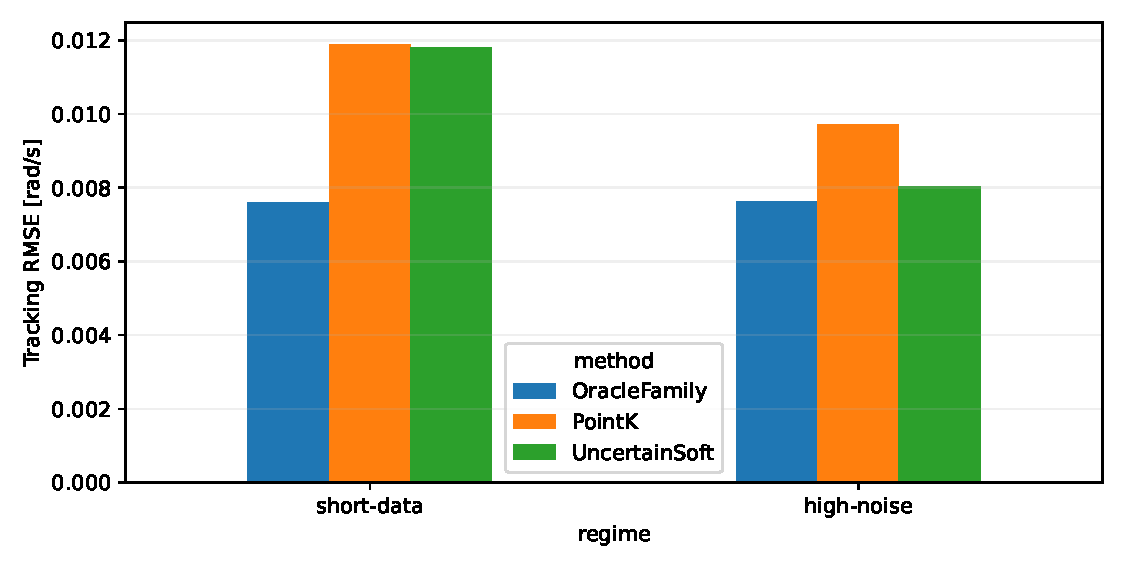
\includegraphics[width=0.78\linewidth]{../results/figures/experiment_9c_uncertainty_groups.pdf}
\caption{Development tracking for ordinary point clustering and uncertainty-
aware soft grouping relative to Oracle family.}
\label{fig:experiment9c}
\end{figure}

\paragraph{Results.}
All 4,200 local fits converge, and all 10,800 nonlinear closed-loop evaluations
are amplitude-feasible and frozen-stable. In the high-noise regime,
uncertainty-aware soft grouping reduces the point-clustering tracking error by
17.27\%. Its oracle cost falls from 27.29\% to 5.31\%, narrowly missing the
predeclared 5\% threshold. BIC selects two groups in every development fleet;
the mean unseen hard-label ARI improves to 0.522, compared with 0.390 for the 9B
point method, but still does not recover the three simulated families.

The 0.25~s regime is qualitatively different. BIC selects $K=1$ in every fleet,
and the proposed method improves point clustering by only 0.65\%. Its 55.45\%
oracle gap shows that uncertainty representation cannot manufacture missing
client-level information. This conclusion is supported by the diagnostics: the
median normalized covariance trace rises from 0.0247 under high noise to 0.141
with 0.25~s records, while the median information-matrix condition number rises
from 55.5 to 248.

\paragraph{Decision.}
The development gate fails in both regimes, so the reserved confirmation seeds
136--145 are not evaluated. This is a deliberate anti-overfitting decision, not
missing evidence. Experiment 9C supports a narrower result: uncertainty-aware
mixture modeling substantially repairs high-noise grouping, but does not resolve
structural non-identifiability from extremely short records. For the paper, the
automatic-grouping claim should remain limited to informative local records.
The next useful experiment should change the information available---for example
active excitation, longer or repeated calibration, or an abstain-and-request-
data policy---rather than applying another clustering rule to the same
uninformative 0.25~s estimates. The untouched seeds remain available for a
genuinely revised method.

\paragraph{Reproducibility.}
The staged protocol is in \path{code/config/experiment_9c.json}; covariance and
mixture routines are in
\path{code/src/federated_lpv/uncertainty_clustering.py}; the experiment driver
is \path{code/experiments/experiment_9c_uncertainty_groups.py}. Development
summaries, cluster diagnostics, gates, and provenance hashes are stored under
\path{results/tables}.
